\subsection{Serverless Architecture}

Kiến trúc Serverless đang trở thành một trong những mô hình tiên quyết và phổ biến nhất để xử lý các workloads của hệ thống Internet of Things (IoT). Theo các nghiên cứu chuyên sâu về kiến trúc đám mây và báo cáo năng lực từ các nhà cung cấp (AWS, Azure), Serverless giải quyết hoàn hảo bài toán biến động dữ liệu (bursty traffic) vốn rất đặc trưng trong hệ thống thiết bị kết nối.

\subsubsection{Mô tả hệ thống}

Kiến trúc Serverless trong IoT hoạt động hoàn toàn dựa trên mô hình \textbf{Tính toán Hướng sự kiện (Event-Driven Compute)}. Trong mô hình này, không có máy chủ nào chạy nền chờ đợi lệnh. Toàn bộ mã nguồn nghiệp vụ chỉ được thực thi khi có một ``sự kiện'' cụ thể từ thiết bị phần cứng được đẩy lên đám mây.

\paragraph*{Sơ đồ kiến trúc}

\begin{figure}[H]
\centering
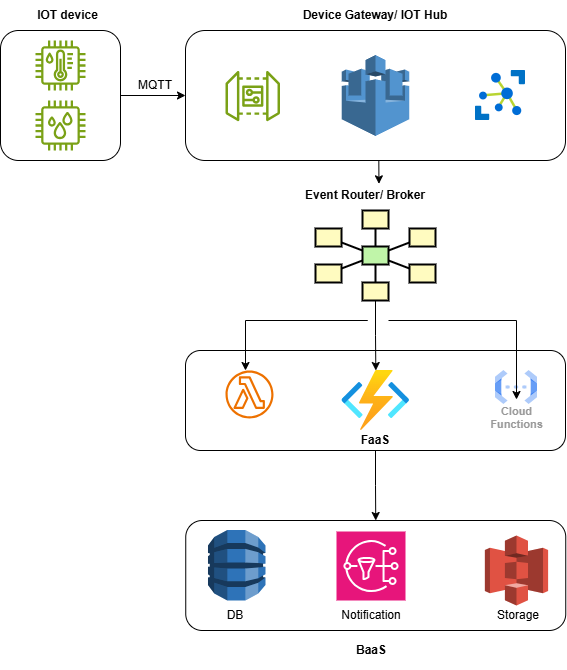
\includegraphics[width=0.9\textwidth]{graphics/serverless-architecture.png}
\caption{Sơ đồ kiến trúc Serverless IoT tiêu biểu}
\label{fig:serverless-architecture}
\end{figure}


\paragraph*{Các thành phần cốt lõi}

Cấu trúc cốt lõi của một hệ thống Serverless IoT bao gồm 4 thành phần chính:

\begin{enumerate}
    \item \textbf{Device Gateway / IoT Hub (Managed Service):}
    \begin{itemize}
        \item Đóng vai trò làm cổng giao tiếp, ví dụ như AWS IoT Core, Azure IoT Hub, Google Cloud IoT.
        \item Quản lý xác thực (Mutual TLS), duy trì kết nối hàng triệu thiết bị cùng lúc bằng các giao thức nhẹ như MQTT, CoAP.
    \end{itemize}

    \item \textbf{Event Router / Broker:}
    \begin{itemize}
        \item Khi thiết bị gửi một bản tin Telemetry hoặc cảnh báo, Broker sẽ đinhn tuyến bản tin này dựa trên các quy tắc sang các dịch vụ xử lý.
    \end{itemize}

    \item \textbf{FaaS (Function-as-a-Service):}
    \begin{itemize}
        \item Trái tim của hệ thống Serverless (ví dụ: AWS Lambda, Azure Functions, Google Cloud Functions).
        \item Mã nguồn được đóng gói thành các hàm nhỏ, phi trạng thái (stateless). Mỗi khi có sự kiện từ thiết bị, nền tảng Cloud sẽ tự động cấp phát một container chớp nhoáng, chạy hàm để xử lý dữ liệu, trả về kết quả và lập tức hủy container đó.
    \end{itemize}

    \item \textbf{BaaS (Backend-as-a-Service):}
    \begin{itemize}
        \item Các dịch vụ lưu trữ phụ trợ được quản lý 100\% như DynamoDB (NoSQL lưu trữ trạng thái thiết bị), Amazon S3 / Blob Storage (lưu trữ firmware), và các dịch vụ cảnh báo (SNS, Firebase Cloud Messaging).
    \end{itemize}
\end{enumerate}

\noindent\textbf{Luồng xử lý tiêu biểu:}\\
\texttt{Cảm biến Nhiệt độ} $\rightarrow$ \texttt{Gửi bản tin MQTT} $\rightarrow$ \texttt{IoT Hub Broker nhận bản tin} $\rightarrow$ \texttt{Kích hoạt hàm Lambda} $\rightarrow$ \texttt{Lambda xử lý, kiểm tra ngưỡng} $\rightarrow$ \texttt{Ghi log vào DynamoDB / Bắn cảnh báo SNS}.

% --------------------------------------------------
\subsubsection{Phân tích sự đánh đổi}
\label{subsec:serverless-tradeoff}

Serverless giải tỏa gánh nặng hạ tầng nhưng cũng buộc các Kiến trúc sư phải chấp nhận những hệ quả kỹ thuật nghiêm ngặt.

\begin{longtable}{c p{4cm} p{4cm} p{4cm}}

\caption{Phân tích đánh đổi kiến trúc Serverless trong IoT}\\

\toprule
\textbf{Chiều Đánh Đổi} & \textbf{Ưu điểm} & \textbf{Hạn chế} & \textbf{Bối cảnh IoT cụ thể} \\
\midrule
\endfirsthead

\toprule
\textbf{Chiều Đánh Đổi} & \textbf{Ưu điểm} & \textbf{Hạn chế} & \textbf{Bối cảnh IoT cụ thể} \\
\midrule
\endhead

\bottomrule
\endfoot

\textbf{Cost}
& \textbf{Pay-as-you-go \& Scale-to-Zero:} Chỉ trả tiền cho từng mili-giây xử lý dữ liệu. Rất hiệu quả cho các thiết bị gửi trạng thái thưa thớt.
& \textbf{Sustained Cost Penalty:} Ở tải liên tục cao, hóa đơn gọi hàm đắt gấp 3--10$\times$ so với Kubernetes/EC2 truyền thống.
& Công tơ nước đọc 1 lần/ngày: chi phí gần bằng 0. Telemetry liên tục 1M sự kiện/ngày: đắt hơn container 5--10$\times$. \\
\hline
\textbf{Latency}
& Phản hồi siêu nhanh đối với các hàm đã được khởi động sẵn (warm start $<$~10ms).
& \textbf{Cold Starts:} 100ms--2s để cấp phát môi trường khi hàm ngưng hoạt động lâu.
& Không chấp nhận được cho yêu cầu $<$~100ms (IIoT safety). Chấp nhận được cho cảnh báo có độ trễ 1--2s. \\
\hline
\textbf{Operations}
& \textbf{Zero Ops:} Không cần DevOps patch OS, tự động mở rộng hoàn hảo.
& \textbf{Vendor Lock-in:} Phụ thuộc sâu vào hệ sinh thái Cloud Provider. Không tinh chỉnh được phần cứng.
& Startup 2 người chạy alerting cho 10K thiết bị mà không cần DevOps. Di chuyển từ AWS sang Azure đòi viết lại IAM + function code. \\
\hline
\textbf{Scalability}
& Tự động scale từ 0 đến hàng triệu instance ngay lập tức.
& \textbf{Concurrency Limits:} AWS Lambda mặc định 1,000 concurrent executions/region. Có thể bị throttle khi spike đột ngột.
& Workload IoT bình thường. Toàn bộ fleet 50K thiết bị reconnect cùng lúc sau mất mạng $\rightarrow$ throttle hàng loạt. \\
\hline
\textbf{Quản lý Trạng thái}
& Bắt buộc thiết kế \textbf{Stateless}, giúp phục hồi sau gián đoạn tức thì. Tách biệt tính toán và dữ liệu.
& \textbf{Phức tạp luồng Stateful:} Theo dõi chuỗi sự kiện (VD: 3 lần vượt ngưỡng liên tiếp) cần Step Functions hoặc Redis bên ngoài.
& Theo dõi trạng thái thiết bị (alert đã gửi chưa?) cần DynamoDB/ElastiCache bên ngoài $\rightarrow$ thêm latency. \\
\hline
\textbf{Giới hạn thực thi}
& Thiết kế cho tác vụ ngắn $\rightarrow$ nhanh, gọn, dễ suy luận.
& AWS Lambda: tối đa 15 phút. Azure Functions: tối đa 10 phút. Không chạy được tác vụ dài.
& ML inference trên tập dữ liệu cảm biến lớn, video transcoding. Data enrichment nhẹ, routing, alerting. \\
\hline
\textbf{Quan sát \& Gỡ lỗi}
& Cloud tự động log cho mỗi lần thực thi (CloudWatch/Monitor).
& \textbf{Mê cung Debug:} Truy vết gói tin đi qua nhiều hàm phân tán rất khó. Cần Distributed Tracing (X-Ray).
& Chuỗi 5 hàm xử lý một alert $\rightarrow$ trace lỗi cần X-Ray/Jaeger. \\

\end{longtable}

% --------------------------------------------------
\subsubsection{Ngữ cảnh áp dụng và Ngưỡng tới hạn}
\label{subsec:serverless-thresholds}

Để kiến trúc tổng thể không rơi vào bẫy ``Anti-pattern'', cần rạch ròi giới hạn của Serverless.

\subsubsection*{Ngữ cảnh áp dụng lý tưởng}

\begin{enumerate}
    \item \textbf{Alerting Pipelines:}
    Mô hình lý tưởng nhất. Cảm biến báo cháy, cảm biến phát hiện rò rỉ hoặc phát hiện rung lắc. Hệ thống hầu như im lặng (Zero Cost) cho đến khi sự cố xảy ra, khi đó Serverless sẽ bung tối đa tài nguyên trong chốc lát để gửi hàng nghìn SMS/Email.

    \item \textbf{Tiền xử lý \& làm sạch dữ liệu:}
    Thiết bị gửi payload dạng chuỗi Hex hoặc Binary nén. Hàm Serverless nhận gói tin, giải mã, áp dụng chuẩn hóa (JSON Schema), và đẩy vào Data Lake hoặc Time-series DB.

    \item \textbf{Quản lý Vòng đời tự động:}
    Tự động chạy các kịch bản Provisioning, đăng ký chứng chỉ bảo mật (Certificates), hoặc cấu hình OTA Update khi thiết bị boot lần đầu tiên.
\end{enumerate}

\paragraph*{Ngưỡng tới hạn (Khi nào hệ thống Serverless sụp đổ?)}

\begin{table}[H]
\centering
\caption{Ngưỡng tới hạn của kiến trúc Serverless trong IoT}
\begin{tabularx}{\textwidth}{c X X X}
\toprule
\textbf{Ngưỡng} & \textbf{Giá trị tới hạn} & \textbf{Hậu quả khi vượt ngưỡng} & \textbf{Giải pháp thay thế} \\
\hline
\textbf{Latency}
  & Closed-loop control $<$~100ms
  & Cold Start (100ms--2s) vi phạm chuẩn an toàn vật lý (Safety-critical).
  & Chuyển sang \textbf{Edge Computing} hoặc container chạy thường trực. \\
\hline
\textbf{Throughput}
  & $>$~1M invocations/ngày liên tục 24/7
  & Chi phí Lambda vượt container 3--10$\times$. VD: Lambda $\sim$\$0.20/1M invocations + compute time vs Fargate $\sim$\$0.04/vCPU-giờ chạy liên tục.
  & Batching vào Kafka/Kinesis $\rightarrow$ xử lý bằng cụm Container (ECS/K8s). \\
\hline
\textbf{Thời gian thực thi}
  & $>$~15 phút (Lambda) / $>$~10 phút (Azure)
  & Timeout tự động ngắt tiến trình giữa chừng.
  & Tách thành pipeline Step Functions hoặc dùng Container/Batch. \\
\hline
\textbf{Concurrency}
  & $>$~1,000 concurrent executions (AWS mặc định)
  & Throttling hàng loạt khi toàn bộ fleet reconnect sau downtime hoặc DDoS.
  & Request quota increase trước hoặc dùng SQS queue làm buffer trước Lambda. \\
\hline
\end{tabularx}
\end{table}

% --------------------------------------------------
\subsubsection{Summary}
\label{subsec:serverless-summary}

Trong bức tranh kiến trúc IoT, \textbf{Serverless} là một ``vũ khí'' cực kỳ sắc bén, làm thay đổi hoàn toàn cục diện chi phí ban đầu và giải phóng đáng kể nguồn lực bảo trì hạ tầng của đội ngũ phát triển. Về cốt lõi, nó tận dụng sức mạnh đàn hồi của đám mây để xử lý các cơn sóng thần dữ liệu (data spikes) --- vốn là đặc tính cốt lõi của hoạt động phần cứng kết nối ngẫu nhiên.

Tuy nhiên, giới khoa học và các chuyên gia kiến trúc đều đồng thuận rằng: \textbf{Serverless KHÔNG phải là một ``Viên đạn bạc'' (Silver Bullet) có thể thay thế mọi thứ.}

\noindent\textbf{Dùng Serverless khi:}
\begin{itemize}
    \item Workload gián đoạn, bursty (cảnh báo, provisioning, ETL ngắt quãng)
    \item Đội ngũ nhỏ ($<$~3 người), không có DevOps
    \item Chi phí tối thiểu là ưu tiên hàng đầu
    \item Độ trễ 1--2s là chấp nhận được
\end{itemize}

\noindent\textbf{Không dùng Serverless khi:}
\begin{itemize}
    \item Telemetry liên tục tần suất cao ($>$~1M msg/ngày sustained)
    \item Safety-critical với yêu cầu $<$~100ms
    \item Tác vụ xử lý dài $>$~15 phút (ML training, video)
    \item Fleet lớn có nguy cơ reconnect storm
\end{itemize}

Sử dụng mô hình này như một mảnh ghép sắc bén ở lớp Xử lý Sự kiện bất đồng bộ, Cảnh báo và Tiền xử lý dữ liệu. Kế đến, họ sẽ điều tiết bằng cách giữ lại Container/Microservices dài hạn cho các luồng Ingestion lưu lượng lớn, và đặc biệt là áp dụng \textbf{Kiến trúc Edge Computing} cho bộ phận ra quyết định yêu cầu độ trễ $<$~100ms. Sự kết hợp khôn khéo này mới tạo nên một vóc dáng hệ thống IoT vững chãi và tối ưu thực sự.
